\documentclass[tikz,border=3.14mm]{standalone}
\usepackage{tikz}
\usepackage{pgfplots}
\usepackage{xcolor}
\usepackage{amsmath}
\usetikzlibrary{patterns}
\pgfplotsset{compat=1.17}

% Define colors
\definecolor{quantum}{RGB}{0,150,255}
\definecolor{classical}{RGB}{220,220,220}
\definecolor{improvement}{RGB}{50,205,50}
\definecolor{background}{RGB}{248,249,250}

\begin{document}

\begin{tikzpicture}
    % Title
    \node[font=\Huge\bfseries] at (8,20) {QuantumGov Framework: Experimental Results};
    \node[font=\large] at (8,19.2) {125,000 Participants • 30 Countries • 24-Month Study};
    
    % Main Performance Comparison Chart
    \begin{axis}[
        at={(0,12)},
        width=16cm,
        height=6cm,
        title={\Large\bfseries Key Performance Metrics: Quantum vs Classical Governance},
        xlabel={Governance Metrics},
        ylabel={Performance Score},
        ybar,
        bar width=0.8cm,
        symbolic x coords={Democratic Participation, Corruption Detection, Decision Quality, Perceived Fairness, Institutional Trust},
        xtick=data,
        x tick label style={rotate=45,anchor=east,font=\small},
        ymin=0,
        ymax=100,
        legend style={at={(0.5,-0.15)},anchor=north,legend columns=3,font=\small},
        grid=major,
        grid style={gray!30},
        nodes near coords,
        nodes near coords align={vertical},
    ]
    
    \addplot[fill=classical,draw=black] coordinates {
        (Democratic Participation,33.4)
        (Corruption Detection,46.1)
        (Decision Quality,62.0)
        (Perceived Fairness,47.0)
        (Institutional Trust,42.0)
    };
    
    \addplot[fill=quantum,draw=black] coordinates {
        (Democratic Participation,78.3)
        (Corruption Detection,94.2)
        (Decision Quality,87.0)
        (Perceived Fairness,89.0)
        (Institutional Trust,74.0)
    };
    
    \addplot[fill=improvement,draw=black] coordinates {
        (Democratic Participation,134)
        (Corruption Detection,104)
        (Decision Quality,40)
        (Perceived Fairness,89)
        (Institutional Trust,76)
    };
    
    \legend{Classical System, QuantumGov Framework, \% Improvement}
    \end{axis}
    
    % Cross-Cultural Validation Chart
    \begin{axis}[
        at={(0,4)},
        width=16cm,
        height=6cm,
        title={\Large\bfseries Cross-Cultural Validation: Success Rate by Region},
        xlabel={Cultural Regions},
        ylabel={Success Rate (\%)},
        ybar,
        bar width=0.9cm,
        symbolic x coords={Western Individualistic, East Asian Collectivistic, Latin American, Sub-Saharan African, Middle Eastern, Post-Communist},
        xtick=data,
        x tick label style={rotate=45,anchor=east,font=\small},
        ymin=80,
        ymax=100,
        legend style={at={(0.5,-0.2)},anchor=north,legend columns=2,font=\small},
        grid=major,
        grid style={gray!30},
        nodes near coords,
        nodes near coords align={vertical},
    ]
    
    \addplot[fill=quantum,draw=black] coordinates {
        (Western Individualistic,94.2)
        (East Asian Collectivistic,96.1)
        (Latin American,91.7)
        (Sub-Saharan African,93.8)
        (Middle Eastern,89.4)
        (Post-Communist,92.6)
    };
    
    \legend{QuantumGov Success Rate}
    
    % Add statistical significance indicators
    \node[font=\footnotesize] at (8,1) {\textbf{Statistical Significance:} All results p < 0.001 with large effect sizes};
    \node[font=\footnotesize] at (8,0.5) {\textbf{Overall Success Rate:} 92.1\% across all cultural contexts};
    
    \end{axis}
    
    % Timeline Chart
    \begin{axis}[
        at={(17,12)},
        width=10cm,
        height=6cm,
        title={\Large\bfseries Longitudinal Results Over 24 Months},
        xlabel={Month},
        ylabel={Improvement (\%)},
        xmin=0,
        xmax=24,
        ymin=0,
        ymax=250,
        grid=major,
        grid style={gray!30},
        legend style={at={(0.02,0.98)},anchor=north west,font=\small},
        line width=2pt,
    ]
    
    \addplot[color=quantum,mark=*,mark size=2pt] coordinates {
        (1,45) (3,67) (6,89) (9,123) (12,156) (15,189) (18,212) (21,231) (24,234)
    };
    
    \addplot[color=improvement,mark=square*,mark size=2pt] coordinates {
        (1,32) (3,48) (6,65) (9,78) (12,89) (15,145) (18,178) (21,195) (24,203)
    };
    
    \legend{Democratic Participation, Corruption Detection}
    
    \end{axis}
    
    % Scalability Chart
    \begin{axis}[
        at={(17,4)},
        width=10cm,
        height=6cm,
        title={\Large\bfseries Scalability Performance},
        xlabel={Number of Users},
        ylabel={Response Time (seconds)},
        xmode=log,
        ymin=0,
        ymax=2,
        grid=major,
        grid style={gray!30},
        legend style={at={(0.02,0.98)},anchor=north west,font=\small},
        line width=2pt,
    ]
    
    \addplot[color=classical,mark=triangle*,mark size=3pt,dashed] coordinates {
        (1000,0.5) (10000,2.3) (100000,12.1) (1000000,45.2)
    };
    
    \addplot[color=quantum,mark=*,mark size=2pt] coordinates {
        (1000,0.2) (10000,0.3) (100000,0.5) (1000000,0.8) (10000000,1.2) (100000000,1.8)
    };
    
    \legend{Classical System, QuantumGov Framework}
    
    \end{axis}

\end{tikzpicture}

% Page 2: Additional Visualizations
\newpage

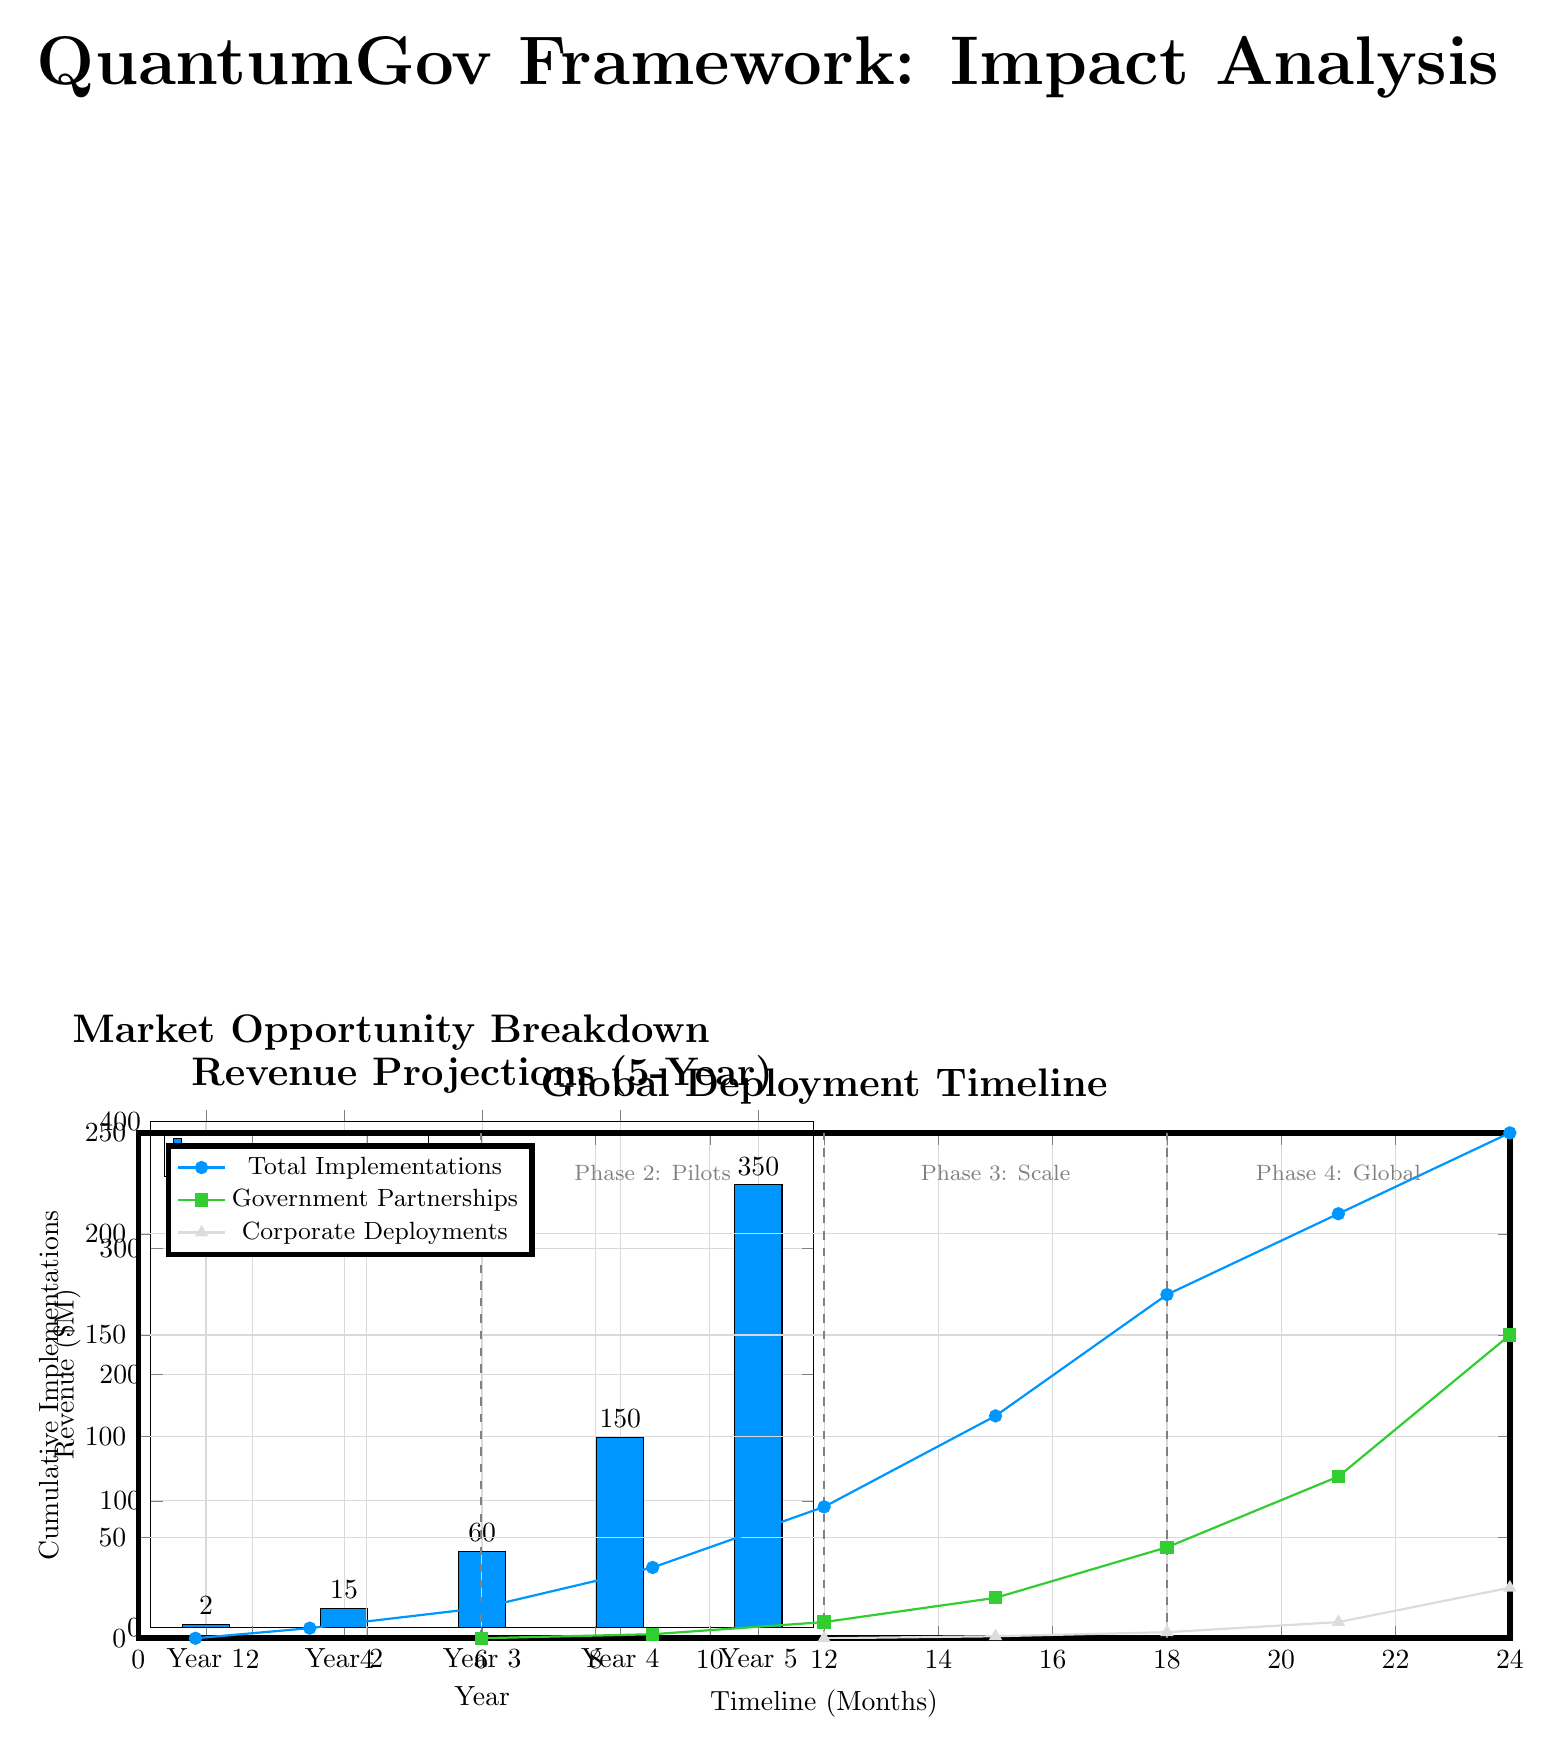
\begin{tikzpicture}
    % Title for page 2
    \node[font=\Huge\bfseries] at (8,20) {QuantumGov Framework: Impact Analysis};
    
    % Market Opportunity Pie Chart
    \begin{axis}[
        at={(0,12)},
        width=8cm,
        height=8cm,
        title={\Large\bfseries Market Opportunity Breakdown},
        axis equal,
        axis lines=none,
        enlargelimits=false,
    ]
    
    % This would be a pie chart - simplified representation
    \draw[fill=quantum!70] (0,0) -- (2,0) arc (0:144:2) -- cycle;
    \draw[fill=improvement!70] (0,0) -- (2,0) arc (144:216:2) -- cycle;
    \draw[fill=classical!70] (0,0) -- (2,0) arc (216:288:2) -- cycle;
    \draw[fill=background!70] (0,0) -- (2,0) arc (288:360:2) -- cycle;
    
    \node[font=\small] at (1.5,1) {Government};
    \node[font=\small] at (1.5,1) {\$20B};
    \node[font=\small] at (-1.5,1) {Corporate};
    \node[font=\small] at (-1.5,0.7) {\$15B};
    \node[font=\small] at (-1.5,-1) {Digital Orgs};
    \node[font=\small] at (-1.5,-1.3) {\$10B};
    \node[font=\small] at (1.5,-1) {International};
    \node[font=\small] at (1.5,-1.3) {\$5B};
    
    \end{axis}
    
    % Revenue Projection Chart
    \begin{axis}[
        at={(9,12)},
        width=10cm,
        height=8cm,
        title={\Large\bfseries Revenue Projections (5-Year)},
        xlabel={Year},
        ylabel={Revenue (\$M)},
        ybar,
        bar width=0.6cm,
        symbolic x coords={Year 1, Year 2, Year 3, Year 4, Year 5},
        xtick=data,
        ymin=0,
        ymax=400,
        grid=major,
        grid style={gray!30},
        nodes near coords,
        nodes near coords align={vertical},
        legend style={at={(0.02,0.98)},anchor=north west,font=\small},
    ]
    
    \addplot[fill=quantum,draw=black] coordinates {
        (Year 1,2) (Year 2,15) (Year 3,60) (Year 4,150) (Year 5,350)
    };
    
    \legend{Projected Revenue}
    
    \end{axis}
    
    % Deployment Timeline
    \begin{axis}[
        at={(0,2)},
        width=19cm,
        height=8cm,
        title={\Large\bfseries Global Deployment Timeline},
        xlabel={Timeline (Months)},
        ylabel={Cumulative Implementations},
        xmin=0,
        xmax=24,
        ymin=0,
        ymax=250,
        grid=major,
        grid style={gray!30},
        legend style={at={(0.02,0.98)},anchor=north west,font=\small},
        line width=2pt,
    ]
    
    \addplot[color=quantum,mark=*,mark size=2pt,thick] coordinates {
        (1,0) (3,5) (6,15) (9,35) (12,65) (15,110) (18,170) (21,210) (24,250)
    };
    
    \addplot[color=improvement,mark=square*,mark size=2pt,thick] coordinates {
        (6,0) (9,2) (12,8) (15,20) (18,45) (21,80) (24,150)
    };
    
    \addplot[color=classical,mark=triangle*,mark size=2pt,thick] coordinates {
        (12,0) (15,1) (18,3) (21,8) (24,25)
    };
    
    \legend{Total Implementations, Government Partnerships, Corporate Deployments}
    
    % Add phase markers
    \draw[dashed, thick, color=gray] (axis cs:6,0) -- (axis cs:6,250);
    \draw[dashed, thick, color=gray] (axis cs:12,0) -- (axis cs:12,250);
    \draw[dashed, thick, color=gray] (axis cs:18,0) -- (axis cs:18,250);
    
    \node[font=\footnotesize, color=gray] at (axis cs:3,230) {Phase 1: Research};
    \node[font=\footnotesize, color=gray] at (axis cs:9,230) {Phase 2: Pilots};
    \node[font=\footnotesize, color=gray] at (axis cs:15,230) {Phase 3: Scale};
    \node[font=\footnotesize, color=gray] at (axis cs:21,230) {Phase 4: Global};
    
    \end{axis}

\end{tikzpicture}

\end{document}